\chapter{Introduksjon}

Utviklingen av skriftspråket har vært et stort bidrag til fremgangen i vårt samfunn. Det er lett å se den enorme innvirkingen dette har hatt. Vi har gått fra å kun kunne dele idéer og tanker muntlig, eller gjennom enkle billedlige fremstillinger, til å metodisk og strukturert kunne skrive det ned og effektivt og presist kunne spre budskapet videre uten forringelse. Våre idéer vil også kunne nå mange flere mottakere samtidig og mottakere som befinner seg mer geografisk spredt. Det vi skriver ned vil også kunne bli lagret over mye lengere tidsperioder til ettertiden uten å miste detaljer i overleveringen slik som kan skje med muntlige overleveringer. Vi bygger opp et kollektivt bibliotek av idéer som vil øke vår kollektive kunnskap og som muliggjør kunnskap som bygger på annen kunnskap i større grad.

\section{Typografi, Gutenberg og orddeling}

Typografien beskjeftiger seg med utformingen og behandlingen av tekst, hvor hovedoppgavene er leselighet og tilpassning av form til innhold. En tekst ønsker å kommunisere et sett med idéer til leseren, hvor typografiens oppgave er å styrke disse idéene i teksten gjennom den visuelle utformingen. Hvis man ikke tar seg bryet med god typografi vil leseren i større grad bli distrahert og leseren vil ledes vekk fra idéene som teksten ønsker å kommunisere. Som det ofte blir sagt; «God typografi er usynlig, dårlig typografi er over alt».

Gjennom hans arbeid med 42-linjersbibelen og samtidig utviklingen av boktrykkerkunsten, fikk Johan Gutenberg (ca. 1400–1468) perfeksjonert mye av det arbeidet som inngår i typografien. Han ønsket å utvikle hurtigere teknikker for produskjon av bøker, hvor resultatet hadde minst like høy kvalitet og visuell skjønnhet som de beste håndproduserte bøkene i hans samtid. 

For at en tekst skal oppfattes som visuelt vakker og ha høy leselighet er spesielt to mål viktig å oppnå: 

Det er spesielt to mål som er viktig å strebe etter, for at en tekst skal oppfattes som estetisk og ha en høy leselighet:

\begin{items}
\item at helheten i teksten har en uniform \textit{farge}\sidenote[-2]{Farge et uttrykk som brukes til å beskrive den helhetlige visuelle opplevelsen av å raskt se over en typsatt side.}, og
\item at teksten er satt med \textit{rette marger}\sidenote{Rette marger er når teksten i sin helhet danner en stram ramme med rette høyre- og venstremarger (slik som denne teksten).}.
\end{items}

Elementer som spiller inn på fargen er: variasjoner i fonttypenes tykkelse og variasjoner i avstanden mellom linjer, ord og bokstaver. Hvis alt dette ikke er tilstrekkelig uniformt kan det oppleves som deler av teksten er luftigere og lysere en andre deler. 

Gutenberg oppnåde gode resultater på de to punktene nevnt over. Første punkt ved å blant annet benytte seg av såkalt \term{hengende punktuering}; hvor enkelte tegn henger litt utenfor tekstens egentlig marg, for å heller skape en mer visuell rett linje som for øyet ser bra ut (se figur \ref{fig:hanging-punctuation}). Enkelte tegn, spesielt punktueringstegn, har mye luft og vil oppleves som et hakk inn om de ikke skyves litt utenfor margen. Bindestrek er et typisk slikt tegn.

\Marginnote{
        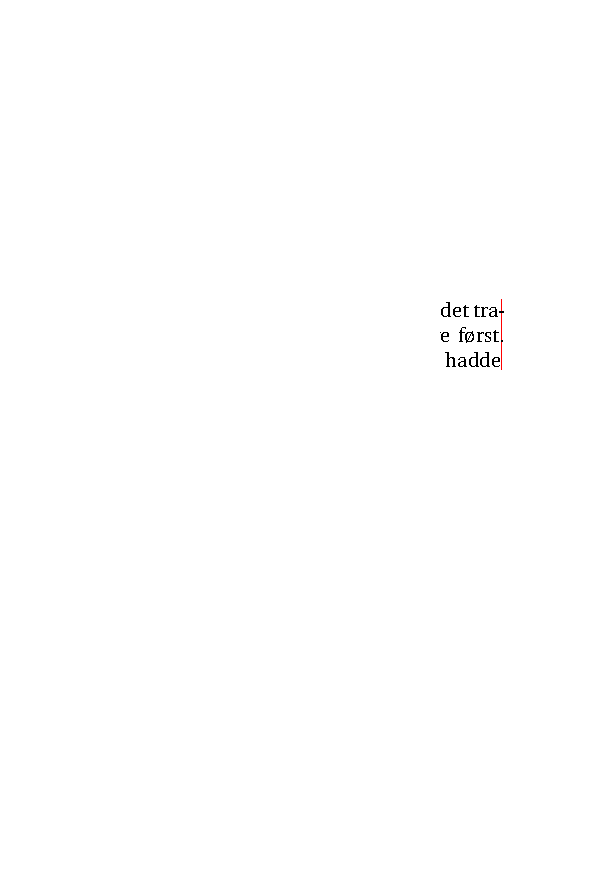
\includegraphics[width=\marginparwidth]{content/examples/hanging-punctuation/hanging-punctuation-crop.pdf}
    \captionof{figure}{Eksempel på hengende punktuering.}
    \label{fig:hanging-punctuation}
}

For å oppnå det andre målet om jevn farge i tekstene sine var det viktig for Gutenberg å få mest mulig uniform avstand mellom ordene i teksten. Det er vanlig når man typsetter at man har fastsatt et visst maks- og minimumsmål for tillatt avstand mellom ord, slik at man har noe spillerom å jobbe med når man skal justere teksten. Men ikke alltid gir dette nok rom, og man trenger andre metoder. Gutenberg gjorde dette ved å skape flere varianter av samme glyph. Typisk da kunne for eksempel en enkelt bokstav «e» ha flere varianter i forskjellige bredder som kunne erstattes for å gi mer spillerom til å justere avstanden mellom ordene. Gutenberg utviklet rundt 290 forskjellige bokstavtyper som han brukte i sin typsetting. Videre vet vi også at orddeling selvfølgelig også er et viktig redksap i å oppnå mest mulig jevn farge.

Selv i dag regnes Gutenbergs 42-linjersbibel som en standard for høykvalitets boktrykk, og flere av de typografiske teknikkene han utviklet er ennå ikke å se i dagens komersielle produkter \cite{thanh2000microtypographic}.


\section{Typografen erstattes av datamaskiner}

Da datamaskinene ble tilstrekkelig kraftig var det naturlig at man ønsket at de tok seg av mye av det typografiske arbeidet. Det ville føre kostnader ned og effektiviteten opp. Enkelte av disse typografiske oppgavene er aspekter som maskiner er mye flinkere enn mennesker til å utføre; for eksempel justering av tekst for å få mest mulig uniforme avstander mellom ord. Et slikt problem kan reduseres til en matematisk funksjon som vekter hver mulige løsning og vi kan da be maskinen om å optimalisere over denne funksjonen. Donald Knuth viser også i sin artikkel \textit{Breaking Paragraphs into Lines*} \cite{knuth1981breaking} at vi nå også kan se på hele avsnitt av gangen når vi skal utføre denne optimaliseringen, i stedet for å bare se på en linje av gangen, som var vanlig når dette arbeidet ble gjort for hånd, eller med de tidligere eksisterende algoritmene.

Et problem som viste seg å være ganske vanskelig for datamaskiner er automatisk deling av ord ved linjeskift, som ikke er løst helt selv i dag. Dette er en svært kompleks lingvistisk operasjon, men for et menneske kan denne oppgaven virke ganske triviell. Vi kjenner til innholdet og betydningen av settningen hvor ordet oppstår og vi har en viss forståelse for reglene som ligger til grunn for orddeling i det språket vi uttrykker oss i. Slik finner vi ganske enkelt rett delepunkt. Men for datamaskiner er det en helt annet kompleksitet. Datamaskiner vil typisk ikke kjenne til den semantiske betydningen av et ord; og for eksempel deling mellom to komponenter i et sammensatt ord blir vanskelig. Det vil også oppstå problemer ved deling av \textit{homonymer}. \sidenote{Homonymer er ord som uttales eller skrives likt.} I slike tilfeller vil konteksten som ordet opptrer bestemme hvordan det skal deles korrekt. For eksempel ordet snekker skal deles som snek-ker (når vi mener håndtverkeren) og snek-k-er (når vi mener båten).

Tekster med lange linjer og kun én kolonne vil typisk ha mindre problemer med å justere teksten og ha færre tilfeller av orddeling ved linjeskift. Derimot tekster hvor det er vanlig med smalere kolonner, som avisartikler, vil dette være et mye mer fremtredene problem. Man får få ord på en linje og får da tilsvarende mindre totalt spillerom i avstanden mellom ordene å jobbe med når teksten skal justeres. Ordene må oftere deles. For å demonstrere problemet ved dette har jeg satt opp tre eksempler som illustrerer dette i figur \ref{fig:three-columns}. 

\begin{SCfigure}
\fcolorbox{red}{white}{
  \parbox{0.27\textwidth}{
  \hyphenpenalty = -1000
 \looseness=-10000
  \spaceskip .5em plus .25em minus .25em
  %\tolerance = -1
  Det var en gang en konge som hadde en datter, og hun var så vakker at hun var navngjeten både vidt og bredt; men hun var så alvorlig av seg at hun aldri kunne le, og så var hun så stor på det at hun sa nei til alle som kom og fridde til henne, og ikke ville hun ha noen, om de var aldri så gilde, enten det var prinser eller herremenn. Kongen var lei av dette for lenge siden, og syntes at hun kunne gifte seg, hun som de andre …
  }
}%
%
\hskip 1em
\fcolorbox{red}{white}{
  \parbox{0.27\textwidth}{
  \hyphenpenalty = 10000
  \looseness=-1
  \spaceskip .5em plus 2em minus .3em
  \tolerance = -1
  Det var en gang en konge som hadde en datter, og hun var så vakker at hun var navngjeten både vidt og bredt; men hun var så alvorlig av seg at hun aldri kunne le, og så var hun så stor på det at hun sa nei til alle som kom og fridde til henne, og ikke ville hun ha noen, om de var aldri så gilde, enten det var prinser eller herremenn. Kongen var lei av dette for lenge siden, og syntes at hun kunne gifte seg, hun som de andre …
  }
}%
%
\hskip 1em
\fcolorbox{red}{white}{
  \parbox{0.27\textwidth}{
  \hyphenpenalty = 10000
  \looseness=-1
  \spaceskip .5em plus .5em minus .15em
  \tolerance = -1
  Det var en gang en konge som hadde en datter, og hun var så vakker at hun var navngjeten både vidt og bredt; men hun var så alvorlig av seg at hun aldri kunne le, og så var hun så stor på det at hun sa nei til alle som kom og fridde til henne, og ikke ville hun ha noen, om de var aldri så gilde, enten det var prinser eller herremenn. Kongen var lei av dette for lenge siden, og syntes at hun kunne gifte seg, hun som de andre …
  }
}

\label{fig:three-columns}
\caption{Første kolonne viser en spalte med tillatt orddeling og noe rom for justering av mellomrom mellom ord. Andre kolonne tillater justering mellom ord, men ingen orddeling. I siste kolonne er også justeringsmulighetene tatt bort. Alle kolonnene er typsatt med med \TeX{}.}
\end{SCfigure}

Siste eksempel er typesatt uten tillatt orddeling og med minimale justeringsmuligheter mellom ordene. Denne teksten ser vi får en fin og jevn farge over seg, men den klarer rett og slett ikke å plassere ordene innenfor den satte rammen med disse strenge kravene, og enkelte ord vil gå utenfor rammen. Ved eksempel to har justeringsmulighetene mellom ordene blitt økt betraktelig. Dette fører til at vi får rette marger, men vi ser fargen i teksten blir ganske ujevn. Det blir flere hvite tomrom i teksten som ikke ser spesielt vakkert ut og kan virke distraherende. Et annet relatert problem som lettere oppstår med løs justering er såkalte \textit{elver} eller \textit{fosser}. \sidenote{Elver og fosser er betegnelsen på hvite tomrom som går vertikalt over flere linjer i teksten. Eksempelvis ser vi dette i figur \ref{fig:three-columns} i midten av andre kolonne.} I første eksempel tillater vi stor grad av orddeling, men med et begrenset spillerom for justering av avstanden mellom ordene. Her får vi både rette marger og en fin farge over teksten.

For å kunne oppnå god typografi i tekster, spesielt i smale kolonner, er det viktig at en algoritme for automatisk orddeling i størst mulig grad finner alle mulige delepunkter i et ord, for å videre kunne gi algortimen som skal dele paragrafer inn i linjer mest mulig å jobbe med. I denne oppgaven vil jeg først se på hvordan algoritmer typisk løser problemet med automatisk orddeling, se i hvor stor grad disse finner delepunkter i ord (og hvor mange feiltreff de har), for så se om det er mulig å utvikle noe som løser dette på en bedre måte — for å igjen kunne typsette tekst bedre.

\section{Oppgavens struktur}

Første del av oppgaven tar for seg orddanning og orddeling: I kapittel to ser vi på ordanning -- hvordan ord er bygget opp, hvordan vi setter dem sammen for å danne nye ord og hvordan vi klassifiserer dem i ordklasser. Dette er relevant for orddelingsreglene. Kapittel tre ser på reglene for orddeling på norsk. I kapittel fire presenteres ulike metoder for automatisk orddeling. Femte kapittel gir en oversikt over tidligere arbeid i fagfelte, både orddelingsalgoritmer og algoritmer for deling av sammensatte ord. Til sist beskrives ressurser som benyttes i del to av oppgaven.

Andre del er en beskrivelse av arbeidet med å utvikle en regelbasert orddeler: Syvende kapittel beskriver arkitektur og implementasjon av en regelbasert orddeler, mens kapittel åtte viser resultater fra testingen av orddeleren samt en diskusjon rundt resultatene.

Tredje og siste del er en oppsummering av oppgaven: I niende og siste kapittel konkluderes oppgaven med en tilbakeblikk på hva vi har lært underveis og et blikk på hvilke muligheter det er for videre arbeid.